\documentclass{article}

\begin{document}


\subsubsection{Muscular activity zone identification by palpation}
	
	When the number of available sEMG electrodes is low, studies have chosen to determine the location of these by palpation. To do this, they first need to determine a set of muscles that they want to measure \cite{ref:Hioki2012} or a set of gesture that must be recognized \cite{ref:Ngeo2014, ref:comp6EMGsetup}. Then, by performing different hand gestures, the zones with the most muscular activities are found by palpation and the electrodes placed at these locations. Visual inspection of the signal given by the electrodes can also by used to find the best spots \cite{ref:Ngeo2014}.
	
	Even if this technique seems easy to use, it is giving poor precision on the exact spots of the electrodes which does not enable to create a reproducible data collection benchmark.
	
	
	\subsubsection{Pre-identified zones giving all the muscular activity of the forearm}
	
	A study from 2018 \cite{ref:identifiedEMGlocation} aimed at determining which zones of the forearm where sufficient to get all the muscular activity of the arm using sEMG electrodes during activities of daily living (ALD) \cite{ref:ADL1}. It started by determining 30 activity spots on the forearm, distributed on a simple grid as shown in figure \ref{fig:forearmActivityZones}.
	
	\begin{figure}[H]
		\centering
		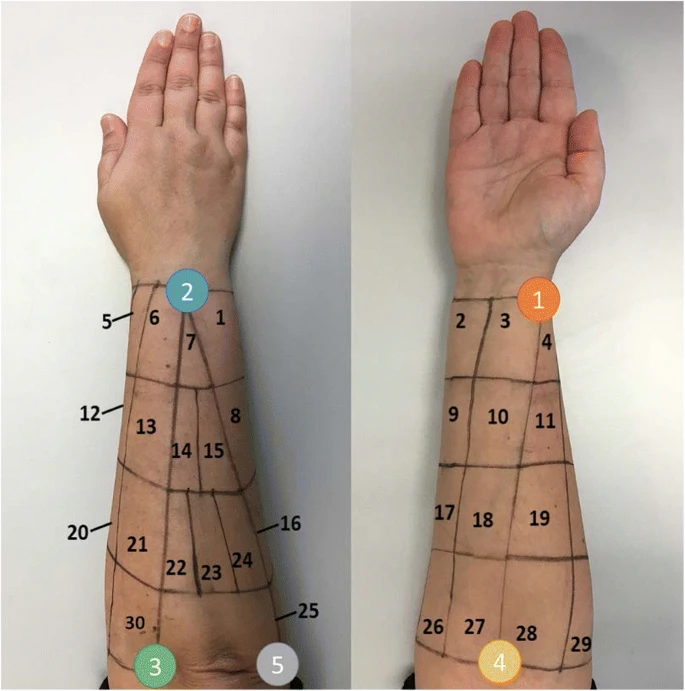
\includegraphics[width=10cm]{images/forearmActivityZones.png}
		\caption{30 spots of muscular activity on the forearm distributed on a grid \cite{ref:identifiedEMGlocation}}
		\label{fig:forearmActivityZones}
	\end{figure}
	
	The researchers recorded 21 ADL (5 sessions of 2 repetition per ADL) on 6 subjects for all 30 spots which gave them 37080 signals of 1000 temporary data which they converted into 30 function of 126000 data. Using functional principal component analysis (FPCA), they simplified the data into a set of 17 reduced variables (RV) responsible for 91\% of the muscular activity. Then, using hierarchical clustering analysis on these 17 RVs, they created a dendrogram, shown in figure \ref{fig:dendrogram}, which allowed them to determine 7 groups of spots with similar muscle activity. Finally, to choose a representative spot of each of the 7 groups, they provide the root mean square of the muscular activity of each spot (figure \ref{fig:MRS}).
	
	\begin{figure}[H] 
		\centering
		\begin{subfigure}{.45 \textwidth}
			\centering
			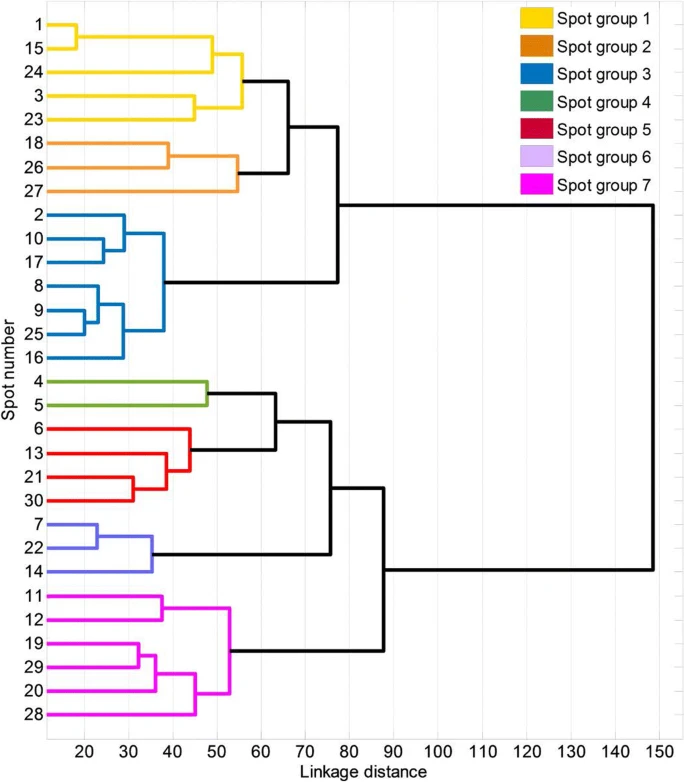
\includegraphics[width=1\linewidth]{images/forearmActivityZonesDendrogram.png}
			\caption{Dendrogram of the 30 activities zones found from hierarchical clustering analysis showing the 7 groups in different colours}
			\label{fig:dendrogram}
		\end{subfigure}%
		\begin{subfigure}{.45 \textwidth}
			\centering
			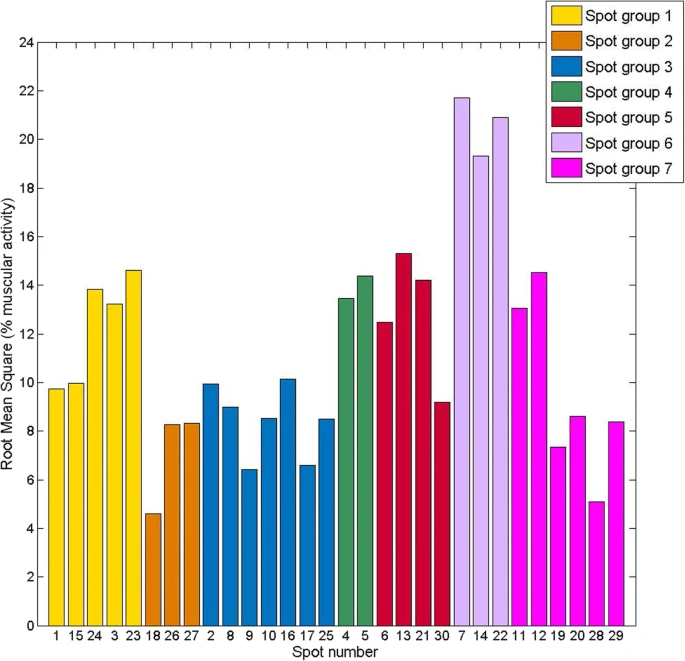
\includegraphics[width=1\linewidth]{images/forearmActivityZonesRMS.png}
			\caption{Root Mean Square of the muscular activities of the 30 activities zones showing the 7 groups in different colours}
			\label{fig:MRS}
		\end{subfigure}
		\caption{Result of the feature selection from the 30 spots of muscular activities on the forearm during activities of daily living \cite{ref:identifiedEMGlocation}}
	\end{figure}
	
	Using this result, we can say that the best 7 spots to place sEMG sensor would be the spots 23, 27, 16, 5, 13, 7 and 12 (ordered by their group number). However, in some circumstances (muscle rehabilitation, ease of placing the electrode), other combination could be considered (as it is the case in the KIN-MUS UJI data set \cite{ref:KinMusUji}).
	
	This method of positioning of the sensors is good for reliability and reproducibility of the data acquisition protocol. However, for a real life application of the hand kinematic prediction (i.e. for a hand myoelectric prosthesis), it might not give a practicable set of locations as they would be really sparse on the whole forearm.
	
	
	\subsubsection{Myoelectric arm band}
	
	The Myoelectric \cite{ref:myoArmBand} arm band was first developed by the company \textit{Thalmic labs}, later rebranded as \textit{North}, after having sold the patents to \textit{CTRL-labs}, a company which was later bought by \textit{Facebook} (\url{https://www.zdnet.com/article/facebook-acquires-ctrl-labs-in-machine-mind-control-research-push/}). It is a device composed of a wristband containing 8 sEMG electrodes (figure \ref{fig:myoArmband}). The main advantages are its price (only 199\$), its ease of use and the fact that it is practicable for real life application such as hand prosthesis control. On the other side, we cannot asses that the location of the sensors is always the same and that they get all the muscular activity needed to accurately predict the hand gestures.
	
	Some studies have used this technologies to do hand gesture classification \cite{ref:Zhang2019} or to use it as an person authentication device \cite{ref:electronics9122143}. Their results were satisfying but the task that had to be done was way simpler than finger joint angles regression. As an example, the study \cite{ref:Zhang2019} only considered 5 different gestures to get a prediction accuracy of 98.7\%.
	
	
	\begin{figure}[H]
		\centering
		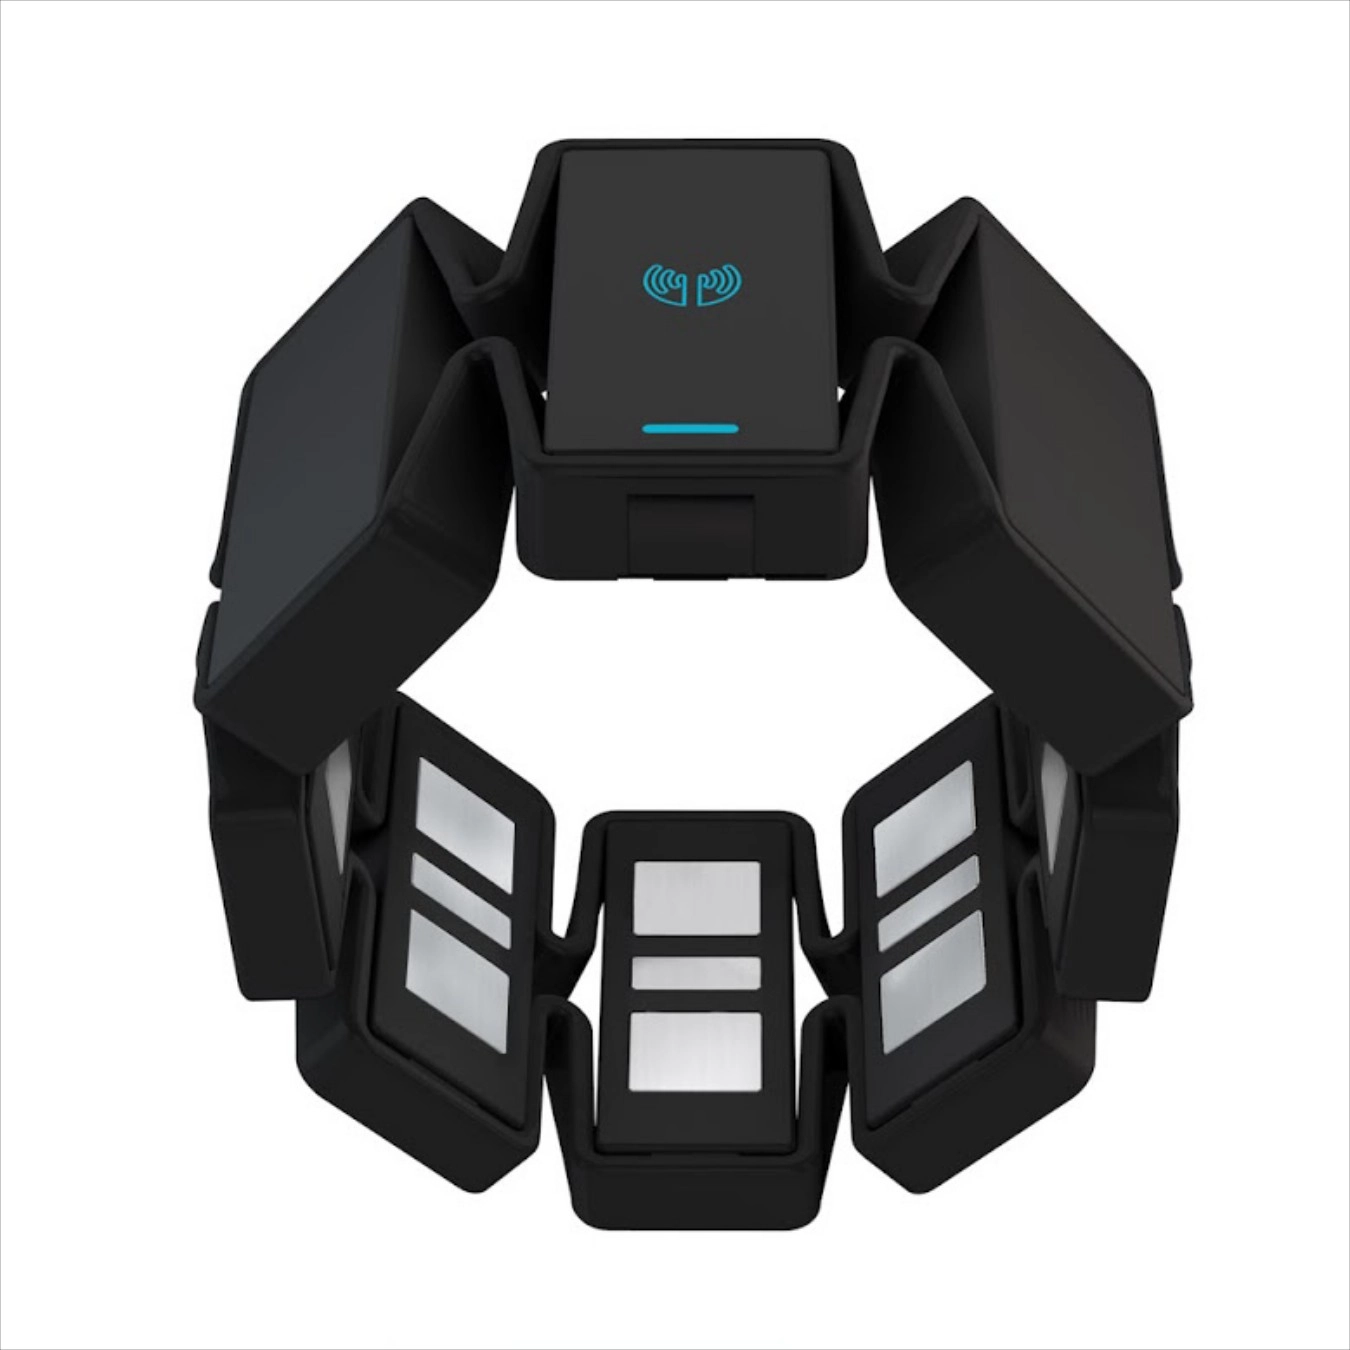
\includegraphics[width=10cm]{images/myoArmBand.png}
		\caption{Picture of the Myo Armband with 8 sEMG sensors \cite{ref:myoArmBand}}
		\label{fig:myoArmband}
	\end{figure}
	
	In 2021, this device is not available in the market anymore. However, a new patent from \textit{Facebook}, release on the 2nd of February 2021 and called \textit{CAMERA - GUIDED INTERPRETATION OF NEUROMUSCULAR SIGNALS } \cite{ref:facebookPatent}, which describes a work similar to this document, shows an improved version of the armband with 16 electrodes. Thus, we can expect similar devices to be released in the market again in the future.
	
\end{document}